\documentclass[11pt,a4paper,twoside,
openright]{book}
\usepackage{fullpage}
\usepackage{amsmath}
\usepackage{mathtools}
\usepackage{amsthm}
\usepackage{amssymb}
\usepackage{amsfonts}
\usepackage{tikz-cd}
\usepackage{cite}
\usepackage{chngcntr}
\usepackage[utf8x]{inputenc}
\usepackage{enumerate}
\usepackage{makeidx}
\usepackage{pgf}
\usepackage{tikz}
\usetikzlibrary{decorations.pathreplacing}
\usetikzlibrary{fadings}
\usetikzlibrary{arrows,shapes,snakes,automata,backgrounds,petri}
\tikzset{basic/.style={draw,fill=blue!50!green!20,
                       text badly centered,minimum width=3em}}
\tikzset{input/.style={basic,circle}}
\tikzset{weights/.style={basic,rectangle,minimum width=2em}}
\tikzset{functions/.style={basic,circle,fill=blue!50!green!20}}
\newcommand{\addsymbol}{\draw[thick] (0.5em,0.5em) -- (0,0.5em) -- 
                        (0,-0.5em) --  (-0.5em,-0.5em)
                        (0em,0.75em) -- (0em,-0.75em)
                        (0.75em,0em) -- (-0.75em,0em);}
\DeclarePairedDelimiter{\ceil}{\lceil}{\rceil}
\renewcommand{\contentsname}{Indice}

\begin{document}

\begin{titlepage}
	
	\begin{figure}
		\centering
		\includegraphics[width=424pt]{tesiSCIENZE_TECNOLOGIE.jpg}%A QUESTO LINK TROVATE I MARCHI PER LA TESI AGGIORNATI E DIVISI PER FACOLTà: http://www.unimi.it/ateneo/37094.htm
		\vspace{0.5 cm}
	\end{figure}
	
%DATO CHE NEI MARCHI SONO GIà PRESENTI SIA IL NOME DELL'UNIVERSITà SIA QUELLO DELLA FACOLTà, NON VANNO RISCRITTI. IN OGNI CASO AGGIUNGO IN COMMENTO COME SAREBBERO:	
%\begin{center}
%	{\Huge \textsc{Università degli Studi di Milano} }\\
%\end{center}
%\begin{center}
%{\Huge Facoltà XXXXX}\\
%\end{center}

\begin{center}
{\LARGE Corso di Laurea F1X}
\end{center}

\begin{center}
\vspace{3 cm}
{\Large \textsc{Compressione di reti neurali in problemi \\ di classificazione e regressione} }
\end{center}
\par
  \vspace{3 cm}
  
  \begin{flushleft}
  		 Relatore:\\Prof. Dario MALCHIODI\\
		 
  		 \noindent Correlatore:\\Dr. Marco FRASCA
  \end{flushleft}
  \vspace{1 cm}
  \begin{flushright}
  	Tesi di Laurea di:\\ Giosuè Cataldo Marinò\\ Matricola: 829404
  \end{flushright}
    	  
\vfill
\begin{center}
	{\large Anno Accademico 2018/2019}
\end{center}

\end{titlepage}


\tableofcontents

\chapter*{Introduzione}
BLABLA
Blablabla said Nobody ~\cite{Nobody06}.
\chapter{Reti Neurali}
\section{Reti Neurali Biologiche}
I neuroni sono delle celle elettricamente attive ed il cervello umano ne contiene circa $10^{11}$. La maggior parte di essi ha la forma indicata in figura~\ref{fig:neurbio}. I dendriti rappresentano gli ingressi del neurone mentre l’assone ne rappresenta l’uscita. La comunicazione tra i neuroni avviene alle giunzioni, chiamate sinapsi. Ogni neurone è tipicamente connesso ad un migliaio di altri neuroni e, di conseguenza, il numero di sinapsi nel cervello supera $10^{14}$.
\begin{figure}[h!]
\begin{center}
\includegraphics[width=200pt]{BioNeuron.png}
\caption{Neurone Biologico~\cite{pict_neur}}
\end{center}
\label{fig:neurbio}
\end{figure}

Ogni neurone si può trovare principalmente in 2 stati: attivo o a riposo. Quando il neurone si attiva esso produce un potenziale di azione (impulso elettrico) che viene trasportato lungo l’assone. Una volta che il segnale raggiunge la sinapsi esso provoca il rilascio di sostanze chimiche (neurotrasmettitori) che attraversano la giunzione ed entrano nel corpo di altri neuroni. In base al tipo di sinapsi, che possono essere eccitatori o inibitori, queste sostanze aumentano o diminuiscono rispettivamente la probabilità che il successivo neurone si attivi. Ad ogni sinapsi è associato un peso che ne determina il tipo e l’ampiezza dell’effetto eccitatore o inibitore. Quindi, in poche parole, ogni neurone effettua una somma pesata degli ingressi provenienti dagli altri neuroni e, se questa somma supera una certa soglia, il neurone si attiva.\\
Ogni neurone, operando ad un ordine temporale del millisecondo, rappresenta un sistema di elaborazione relativamente lento; tuttavia, l’intera rete ha un numero molto elevato di neuroni e sinapsi che possono operare in modo parallelo e simultaneo, rendendo l’effettiva potenza di elaborazione molto elevata. Inoltre la rete neurale biologica ha un’alta tolleranza ad informazioni poco precise (o sbagliate), ha la facoltà di apprendimento e generalizzazione.

\section{Reti Neurali Artificiali}
Ci concentreremo su una classe particolare di modelli di reti neurali: le reti a catena aperta (feedforward). Queste reti possono essere viste come funzioni matematiche non lineari che trasformano un insieme di variabili indipendenti $x = (x_{1}, ... , x_{d})$, chiamate ingressi della rete, in un insieme di variabili dipendenti $y = (y_{1}, ... , y_{c})$, chiamate uscite della rete. La precisa forma di queste funzioni dipende dalla struttura interna della rete e da un insieme di valori $w = (w_{1}, ... , w_{d})$, chiamati pesi. Possiamo quindi scrivere la funzione della rete nella forma $y = y(x; w)$ che denota il fatto che $y$ sia una funzione di $x$ parametrizzata da $w$.

\begin{figure}[h!]
\begin{center}
\tikzset{basic/.style={draw,fill=white,text width=1em,text badly centered}}
\tikzset{input/.style={basic,circle}}
\tikzset{weights/.style={basic,rectangle}}
\tikzset{functions/.style={basic,circle,fill=white}}
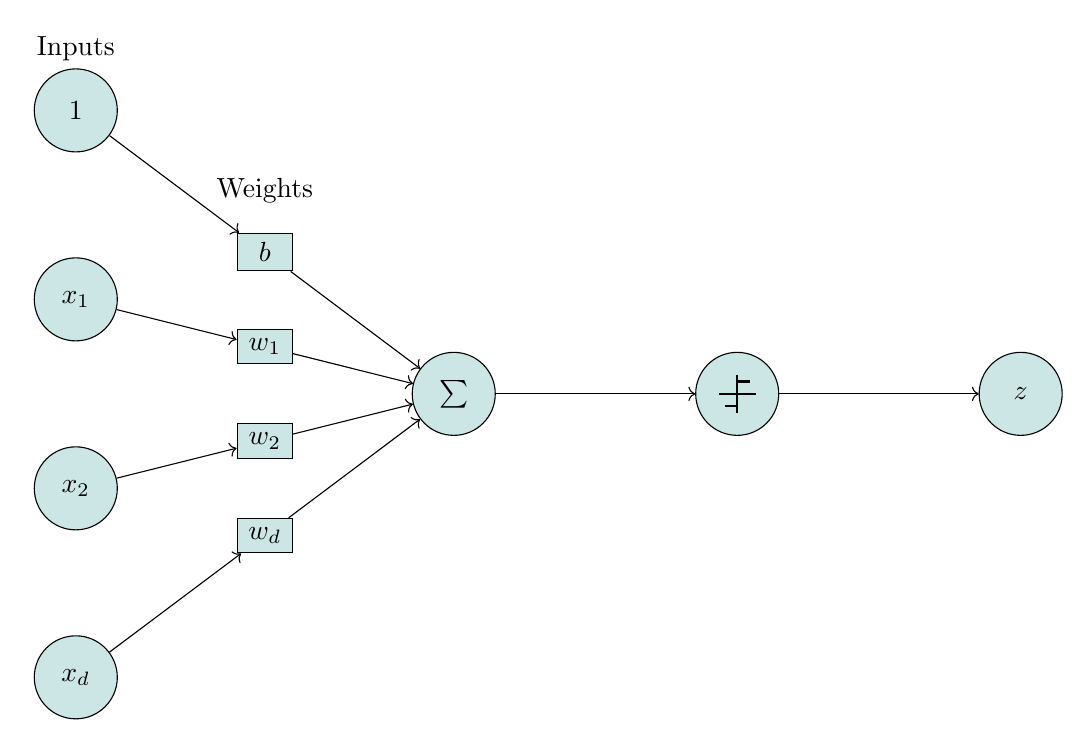
\begin{tikzpicture}[scale=1.2]
    \foreach \h [count=\hi ] in {$x_d$,$x_2$,$x_1$,$1$}{%
          \node[input] (f\hi) at (0,\hi*2cm-5 cm) {\h};
        }
    \node[input] (z) at (10,0) {$z$};
    \node[functions] (sum) at (4,0) {$\sum$};
    \foreach \h [count=\hi ] in {$w_d$,$w_2$,$w_1$,$b$}{%
          \path (f\hi) -- node[weights] (w\hi) {\h} (sum);
          \draw[->] (f\hi) -- (w\hi);
          \draw[->] (w\hi) -- (sum);
        }        
    \node[functions] (step) at (7,0) {};
       \begin{scope}[xshift=7cm,scale=.75]
         \addsymbol
       \end{scope}
    \draw[->] (sum) -- (step);
    \draw[->] (step) -- (z);%++(1,0);
    % Labels
    \node[above=.5cm]  at (f4) {Inputs};
    \node[above=.5cm] at (w4) {Weights};
    
\end{tikzpicture}
\end{center}
\caption{Modello di McCulloch-Pitts}
\label{fig:mcpitts}
\end{figure}
\subsection*{Modello di McCulloch-Pitts}

Un semplice modello matematico di un singolo neurone è quello rappresentato in figura~\ref{fig:mcpitts} ed è stato proposto da McCulloch e Pitts ~\cite{McCulloch:1943aa} alle origini delle reti neurali. Esso può essere visto come una funzione non lineare che trasforma le variabili di ingresso $x_{1}, ..., x_{d}$ nella variabile di uscita $z$. Nell’elaborato ci riferiremo a questo modello come unità di elaborazione, o semplicemente unità.
In questo modello, viene effettuata la somma ponderata degli ingressi, usando come pesi i valori $w_{1}, ..., w_{d}$ (che sono analoghi alle potenze delle sinapsi nella rete biologica), ottenendo così:
\begin{equation}
a = \sum\limits_{i=1}^d w_{i}x_{i}+b
\label{som+b}
\end{equation}

dove il parametro $b$ viene chiamato bias (corrisponde alla soglia di attivazione del neurone biologico). Se definiamo un ulteriore ingresso $x_{0}$, impostato costantemente a 1, possiamo scrivere l'equazione~\eqref{som+b} come:
\begin{equation}
a = \sum\limits_{i=0}^d w_{i}x_{i}
\label{som}
\end{equation}
dove $x_{0}$ = 1. Precisiamo che i valori dei pesi possono essere di qualsiasi segno, che dipende dal tipo di sinapsi. L’uscita $z$ (che può essere vista come tasso medio di attivazione del neurone biologico) viene ottenuta applicando ad a una trasformazione non lineare $g()$, chiamata funzione di attivazione, ottenendo 
\begin{equation}
z=g(a)=g\left( \sum\limits_{i=1}^d w_{i}x_{i} \right).
\label{act+som}
\end{equation}
Il modello originale di McCulloch-Pitts usava la funzione gradino
\begin{equation}
g(a)=
\begin{cases}
1 &\text{ se } a\geq0 \\
-1 &\text{ altrimenti}
\end{cases}
\label{act+som}
\end{equation}

\section{Addestramento della rete}
Abbiamo detto che una rete neurale può essere rappresentata dal modello matematico $y = y(x; w)$, che è una funzione di $x$ parametrizzata dai pesi $w$. Prima di poter utilizzare questa rete, dobbiamo identificare il modello, ovvero dobbiamo determinare tutti i parametri $w$. Il processo di determinazione di questi parametri è chiamato addestramento e può essere un’azione molto intensa dal punto di vista computazionale. Tuttavia, una volta che sono stati definiti i pesi, nuovi ingressi possono essere processati molto rapidamente.
Per addestrare una rete abbiamo bisogno di un insieme di esempi, chiamato insieme di addestramento (\textit{training set}), i cui elementi sono coppie $(x^{q}, t^{q})$, $q = 1, ..., n$, dove $t^{q}$ rappresenta il valore di uscita desiderato, chiamato target, in corrispondenza del ingresso $x^{q}$. 
L’addestramento consiste nella ricerca dei valori per i parametri $w$ che minimizzano un’opportuna funzione di errore. Ci sono diverse forme di questa funzione, la più usata risulta essere la somma dei quadrati residui. I residui sono definiti come:
\begin{equation}
r_{qk} = y_{k}\left(x^{q}; w\right) - t^{q}_{k}
\label{res}
\end{equation}
La funzione di errore E risulta allora essere:
\begin{equation}
E = \sum\limits_{q=1}^n \sum\limits_{k=1}^c r_{qk}^{2}
\label{quadres}
\end{equation}
é facile osservare che E dipende da $x^{q}$ e da $t^{q}$ che sono valori noti e da $w$ che è incognito, quindi E è in realtà una funzione dei soli pesi $w$.

\section{Funzioni di attivazione}
Le funzioni di attivazione sono equazioni matematiche che determinano l'output di una rete neurale.
Le funzioni utilizzate principalmente negli esperimenti di questo elaborato sono tre: \textit{sigmoid}, \textit{ReLU} (\textit{Rectified Linear Units}) e \textit{Leaky-ReLU}.
Le funzioni di attivazione sono non-lineari e la loro derivata è calcolabile in modo analitico per velocizzare la computazione.

\begin{equation}
sigmoid(a) = \frac{1}{1+e^{-x}} \qquad
sigmoid'(a) = sigmoid(a)(1-sigmoid(a))
\label{sigmoid}
\end{equation}

\begin{equation}
ReLU(a) = \max(0,a) \qquad
ReLU'(a) = \begin{cases}
1 &\text{ se } a\geq0 \\
0 &\text{ altrimenti}
\end{cases}
\label{relu}
\end{equation}

\begin{equation}
Leaky-ReLU(a) = \begin{cases}
a &\text{ se } a\geq0 \\
- \alpha a &\text{ altrimenti}
\end{cases} \qquad
Leaky-ReLU'(a) = \begin{cases}
1 &\text{ se } a\geq0 \\
\alpha &\text{ altrimenti}
\end{cases}
\label{lrelu}
\end{equation}
dove $\alpha$ è un parametro numerico.

La scelta della funzione è guidata dal tipo di problema che si vuole affrontare, per esempio se vogliamo un output compreso tra 0 e 1 sarà più adeguato utilizzare una funzione \textit{sigmoid} rispetto ad una \textit{ReLU}.



\section{MultiLayer Perceptron}
\subsection{Architettura del modello MLP}
\paragraph{Modello a uno strato}
\def\layersep{2.5cm}

\begin{figure}[h!]
\begin{center}
\begin{tikzpicture}[shorten >=1pt,->,draw=black!50, node distance=\layersep]
    \tikzstyle{every pin edge}=[<-,shorten <=1pt]
    \tikzstyle{neuron}=[basic,circle,fill=black!25,minimum size=17pt,inner sep=0pt]
    \tikzstyle{input neuron}=[neuron, fill=white];
    \tikzstyle{output neuron}=[neuron, fill=white];
    \tikzstyle{hidden neuron}=[neuron, fill=white];
    \tikzstyle{annot} = [text width=4em, text centered]

    % Draw the input layer nodes
    \foreach \name / \y in {0,...,3}
    % This is the same as writing \foreach \name / \y in {1/1,2/2,3/3,4/4}
        \node[input neuron] (I-\name) at (0,-\y-1) {$x_\y$};
	\node[input neuron] (I-d) at (0,-4-1) {$x_d$};
    
    %\node[annot,pin={[pin edge={->}]right:bias}, left of=I-0] (O) {};
	\node[annot,pin={[pin edge={->}]below:},above of=I-0, node distance=1.5cm] {$bias$};
    % Draw the output layer node
    \node[output neuron, right of=I-1] (O) {$z_1$};
    \node[output neuron, right of=I-3] (O2) {$z_m$};

    % Connect every node in the input layer with every node in the
    % hidden layer.
    \foreach \source in {0,...,3}
    	\path (I-\source) edge (O);
    \foreach \source in {0,...,3}
    	\path (I-\source) edge (O2);
    \path (I-d) edge (O);
    \path (I-d) edge (O2);

    % Annotate the layers
    
    %\node[annot, node distance=1cm] (input) {Input layer};
    \node[annot, below of=I-d, node distance=2cm] (input) {Input layer};
    \node[annot, right of=input] {Output layer};
\end{tikzpicture}
\end{center}
\caption{MLP a uno strato}
\label{fig:MLP1}
\end{figure}
Nella sezione precedente abbiamo trattato la singola unità di elaborazione descritta dall'equazione~\eqref{act+som}. Consideriamo ora un insieme di $m$ unità, con ingressi comuni, otteniamo una rete neurale a singolo strato come in figura~\ref{fig:MLP1}. Le uscite di questa rete sono date da
\begin{equation}
z_j = g\left(\sum\limits_{i=0}^d w_{ji}x_i\right), \quad
j=1,..,m
\label{rete1}
\end{equation}
dove $w_{ij}$ rappresenta il peso che connette l'ingresso $i$ con l'uscita $j$; $g()$ è una funzione di attivazione. $x_0=1$ per utilizzare l'equazione semplificata.

\paragraph{Modello a due strati}
\begin{figure}[ht!]
\begin{center}
\def\layersep{1.5cm}

\begin{tikzpicture}[
   shorten >=1pt,->,
   draw=black!50,
    node distance=\layersep,
    every pin edge/.style={<-,shorten <=1pt},
    neuron/.style={circle,basic,fill=black!25,minimum size=17pt,inner sep=0pt},
    input neuron/.style={neuron, fill=white},
    output neuron/.style={neuron, fill=white},
    hidden neuron/.style={neuron, fill=white},
    annot/.style={text width=4em, text centered}
]
	
	\foreach \name / \y in {0,...,2}
    % This is the same as writing \foreach \name / \y in {1/1,2/2,3/3,4/4}
        \node[input neuron] (I-\name) at (0,-\y-1) {$x_\y$};
	\node[input neuron] (I-d) at (0,-3-1) {$x_d$};
    % Draw the input layer nodes
    %\foreach \name / \y in {1,...,4}
    % This is the same as writing \foreach \name / \y in {1/1,2/2,3/3,4/4}
    %    \node[input neuron, pin=left:Input \#\y] (I-\name) at (0,-\y) {};

    % set number of hidden layers
    \newcommand\Nhidden{1}

    % Draw the hidden layer nodes
    
	\foreach \y in {0,...,4}
    % This is the same as writing \foreach \name / \y in {1/1,2/2,3/3,4/4}
        \node[input neuron] (H-\y) at (\layersep,-\y) {$z_\y$};
	\node[input neuron] (H-m) at (\layersep,-5) {$z_m$};    
    
    %\foreach \N in {1,...,\Nhidden} {
    %   \foreach \y in {1,...,5} {
    %      \path[yshift=0.5cm]
    %          node[hidden neuron] (H\N-\y) at (\N*\layersep,-\y cm) {};
    %       }
    \node[annot,below of=H-m, node distance=2cm] (hl) {Hidden layer};
    
	\node[annot,pin={[pin edge={->}]below:},above of=I-0] {$bias$};
	\node[annot,pin={[pin edge={->}]below:},above of=H-0] {$bias$};
    % Draw the output layer node
    \node[input neuron, right of=H-2] (O) {$y_1$};
    \node[input neuron, below of=O] (Oc) {$y_c$};

    % Connect every node in the input layer with every node in the
    % hidden layer.
    \foreach \source in {0,...,2}
        \foreach \dest in {0,...,4}
            \path (I-\source) edge (H-\dest);
	\foreach \dest in {0,...,4}     
     	\path (I-d) edge (H-\dest);  
    \foreach \source in {0,1,2,d}
            \path (I-\source) edge (H-m);      

    % connect all hidden stuff
   % \foreach [remember=\N as \lastN (initially 1)] \N in {1}%{2,...,\Nhidden}
    %   \foreach \source in {1,...,5}
     %      \foreach \dest in {1,...,5}
      %         \path (H\lastN-\source) edge (H\N-\dest);

    % Connect every node in the hidden layer with the output layer
    \foreach \source in {0,...,4}
        \path (H-\source) edge (O);
	\path (H-m) edge (O);
    % Annotate the layers
    \foreach \source in {0,...,4}
        \path (H-\source) edge (Oc);
	\path (H-m) edge (Oc);

    \node[annot,left of=hl] {Input layer};
    \node[annot,right of=hl] {Output layer};
\end{tikzpicture}
\caption{MLP a due strati}
\label{fig:MLP2}
\end{center}
\end{figure}
Per ottenere reti più potenti è necessario considerare reti aventi più strati chiamate \textit{multilayer perceptron}. Le unità centrali rappresentano lo strato nascosto (\textit{hidden}) perchè il valore di attivazione delle singole unità di questo strato non sono misurabili dall'esterno. L'attivazione di queste unità è data dall'equazione~\eqref{rete1}. Le uscite della rete vengono ottenute tramite una seconda trasformazione, analoga alla prima, sui valori $z_j$ ottenendo
\begin{equation}
y_k = \tilde{g}\left(\sum\limits_{j=0}^m \tilde{w}_{kj}z_i\right), \quad
k=1,..,c
\label{rete2}
\end{equation}
dove $\tilde{w}_{kj}$ rappresenta il peso del secondo strato che connette l'unità nascosta $j$ all'unità di uscita $k$. Sostituendo l'equazione~\eqref{rete1} nell'equazione~\eqref{rete2} otteniamo:
\begin{equation}
y_k = \tilde{g}\left( \sum\limits_{j=0}^m \tilde{w}_{kj}g\left(\sum\limits_{i=0}^d w_{ji}x_i\right) \right), \quad
k=1,..,c
\label{rete2.1}
\end{equation}
La funzione di attivazione $\tilde{g}$, applicata alle unità di uscità può essere diversa dalla funzione di attivazione $g$, applicata alle unità nascoste.

Per ottenere una capacità di rappresentazione universale, la funzione di attivazione $g$ delle unità nascoste deve essere scelta non lineare. Se $g$ e $\tilde{g}$ fossero entrambe lineari l'equazione~\eqref{rete2.1} diventerebbe un prodotto tra matrici, che è esso stesso una matrice. Inoltre, come vedremo più avanti, le funzioni di attivazione devono essere differenziabili.
\subsection{Addestramento}
L'addestramento consiste nella ricerca dei valori $\textbf{w}=(w_1,..,w_d)$ che minimizzano la funzione di errore $E(\textbf{w})$.
La ricerca del minimo avviene in modo iterativo partendo da un valore iniziale $\textbf{w}$, scelto in modo casuale o tramite un criterio. Alcuni algoritmi trovano il minimo locale più vicino al punto iniziale, mentre altri riescono a trovare il minimo globale.

Diversi algoritmi di ricerca del punto minimo fanno uso delle derivate parziali della funzione di errore $E$, ovvero del suo vettore gradiente $\nabla E$. Questo vettore indica la direzione ed il verso di massima crescita di $E$ nel punto $\textbf{w}$.
\subsection*{Error back-propagation~\cite{Rumelhart20081B}}
Consideriamo come funzione errore la somma dei quadrati residui~\eqref{quadres}. 
\begin{equation}
E = \sum\limits_{q=1}^n E^{q} \qquad
E^q = \sum\limits_{k=1}^c [y_k (x^q;w) - t_{k}^{q}]^2
\label{resq}
\end{equation}

Possiamo vedere $E$ come somma di $E^q$ che corrisponde alla coppia $(x^q,t^q)$. Grazie alla linearità della derivazione possiamo calcolare la derivata di $E$ come somma delle derivate dei termini $E^q$. Omettiamo l'indice $q$, i passaggi che seguiranno si riferiranno ad un singolo caso $q$ ma le operazioni sono fatte per ogni valore di $q$. Consideriamo un esempio di rete neurale MLP con 1 strato hidden.

\begin{equation}
y_k=\tilde{g}(\tilde{a}_k) \qquad
 a_k=\sum\limits_{j=0}^m \tilde{w}_{kj}z_j
\label{ak}
\end{equation}
La derivata di $E^q$ rispetto ad un generico peso $w_{kj}$ dello strato hidden:
\begin{equation}
\frac{\partial E^q}{\partial \tilde{w}_{kj}}=\frac{\partial E^q}{\partial \tilde{a}_k}\frac{\partial \tilde{a}_k}{\partial w_{kj}}
\label{chain}
\end{equation}
Con l'equazione~\eqref{ak} troviamo:
\begin{equation}
\frac{\partial \tilde{a}_k}{\partial \tilde{w}_{kj}}=z_j
\label{chain1}
\end{equation}
Dalle equazioni~\eqref{ak} e~\eqref{resq}:
\begin{equation}
\frac{\partial E^q}{\partial \tilde{a}_k}=\tilde{g}'(\tilde{a}_k)[y_k-t_k]
\label{chain2}
\end{equation}
Otteniamo quindi:
\begin{equation}
\frac{\partial E^q}{\partial w_{kj}}=\tilde{g}'(\tilde{a}_k)[y_k-t_k]z_j.
\label{chain2}
\end{equation}
Definendo
\begin{equation}
\tilde{\delta}_k = \frac{\partial E^q}{\partial \tilde{a}_k}=\tilde{g}'(\tilde{a}_k)[y_k-t_k]
\label{delta}
\end{equation}
otteniamo una semplice espressione per la derivata di $E^q$ rispetto a $w_{kj}$:
\begin{equation}
\frac{\partial E^q}{\partial \tilde{w}_{kj}}=\tilde{\delta}_k z_j.
\label{deltaz}
\end{equation}



Per quanto riguarda le derivate rispetto ai pesi del primo strato riscriviamo:
\begin{equation}
z_j=g(a_j) \qquad
 a_j=\sum\limits_{i=0}^d w_{ji}x_i.
\label{aj}
\end{equation}
Possiamo quindi scrivere la derivata come
\begin{equation}
\frac{\partial E^q}{\partial w_{ji}}=\frac{\partial E^q}{\partial a_j}\frac{\partial a_j}{\partial w_{ji}}
\label{chain3}
\end{equation}
In modo analogo, osservando~\eqref{aj}, troviamo:
\begin{equation}
\frac{\partial a_j}{\partial w_{ji}}=x_i
\label{chain4}
\end{equation}
Per il calcolo della derivata di $E^q$ rispetto ad $a_j$, usando la \textit{chain-rule} abbiamo che:
\begin{equation}
\frac{\partial E^q}{\partial a_j}=\sum\limits_{k=1}^c \frac{\partial E^q}{\partial \tilde{a}_k}\frac{\partial \tilde{a}_k}{\partial a_j}
\label{chain5}
\end{equation}
dove la derivata di $E^q$ rispetto ad $\tilde{a}_k$ è data dall'equazione~\eqref{chain2}, mentre la derivata di $\tilde{a}_k$ rispetto ad $a_j$ la troviamo usando le equazioni~\eqref{ak} e~\eqref{aj}:
\begin{equation}
\frac{\partial \tilde{a}_k}{\partial a_j}=\tilde{w}_{kj}g'(a_j).
\label{chain6}
\end{equation}
Usando le equazioni~\eqref{delta},~\eqref{chain5} e~\eqref{chain6}:
\begin{equation}
\frac{\partial E^q}{\partial a_{j}}=g'(a_j)\sum\limits_{k=1}^c \tilde{w}_{kj}\tilde{\delta}_k.
\label{chain7}
\end{equation}
Possiamo quindi riscrivere l'equazione~\eqref{chain3}:
\begin{equation}
\frac{\partial E^q}{\partial w_{ji}}=g'(a_j)x_i\sum\limits_{k=1}^c w_{kj}\delta_k
\label{chain8}
\end{equation}
Come abbiamo fatto nell'equazione~\eqref{delta}, poniamo
\begin{equation}
\delta_j = \frac{\partial E^q}{\partial a_j}=g'(a_j)\sum\limits_{k=1}^c \tilde{w}_{kj}\tilde{\delta}_k
\label{delta2}
\end{equation}
Ottenendo infine
\begin{equation}
\frac{\partial E^q}{\partial w_{ji}}=\delta_j x_i
\label{deltax}
\end{equation}
che ha la stessa semplice forma dell'equazione~\eqref{deltaz}.
Elenchiamo quindi i passi da seguire per valutare la derivata della funzione E:
\begin{itemize}
\item Per ogni coppia $(\textbf{x}^q,\textbf{t}^q)$ valutare le attivazioni delle unità nascoste e di uscita usando le equazioni~\eqref{aj} e~\eqref{ak};
\item Valutare il valore $\tilde{\delta}_k$ per $k=1,..,c$ usando equazione~\eqref{delta};
\item Valutare il valore $\delta_j$ per $j=1,..,m$ usando equazione~\eqref{delta2};
\item Valutare il valore di $E^q$ usando le equazioni~\eqref{deltax} e~\eqref{deltaz};
\item Ripetere i passi precedenti per ogni coppia $(\textbf{x}^q,\textbf{t}^q)$ del \textit{training set} e sommare tutte le derivate per ottenere la derivata della funzione errore $E$.
\end{itemize}

Dopo il calcolo delle derivate i pesi di ogni strato verranno aggiornati come:
\begin{equation}
w_{ij}^{(t)}=w_{ij}^{(t-1)} + \Delta w_{ij}^{(t)},
\label{update_w_ij}
\end{equation}
\begin{equation}
\Delta w_{ij}^{(t)} = -\eta \nabla E(w_{ij}^{(t)}),
\label{deltawij}
\end{equation}
dove $\eta$ è il coefficiente di apprendimento (\textit{learning rate}), più $\eta$ è grande più imparera velocemente.
Questo verrà ripetuto iterativamente ogni epoca, dove con epoca intendiamo la visione dell'intero \textit{training set}.
L'aggiornamento dei pesi durante ogni epoca può avvenire dopo ogni elemento (\textit{online}), dopo tutti gli elementi (\textit{batch}) o dopo un numero parametrico di esempi (\textit{mini-batch}).
Negli esperimenti di questo elaborato viene utilizzata la modalità \textit{mini-batch} perchè permette al modello di convergere più velocemente.

Per migliorare la convergenza della rete abbiamo utilizzato la versione di discesa del gradiente con \textit{momento}~\cite{journals/nn/Qian99}.
In questa versione l'equazione~\eqref{deltawij} diventa:
\begin{equation}
w_{ij}^{(t)}=- \eta \nabla E(w_{ij}^{(t)}) + \mu \Delta w_{ij}^{(t-1)}
\label{momentum}
\end{equation}
dove $\mu$ è un parametro aggiuntivo nell'intervallo $[0,1)$ che valorizza quanto considerare il gradiente dell'epoca precedente. 
Questo tipo di aggiornamento accelererà la convergenza se il verso del gradiente è lo stesso dell'epoca precedente. 

\subsection*{Stopping}
In questa sezione vogliamo rispondere alla domanda: "quando fermiamo l'addestramento?". Negli esperimenti sono stati utilizzati diversi criteri, quali:
\begin{itemize}
\item Stop dopo un numero prefissate di epoche;
\item Stop dopo che l'errore/accuratezza non migliora rispetto all'epoca precedente;
\item Stop dopo che l'errore/accuratezza non migliora rispetto all'epoca precedente con \textit{patience}, ovvero che si aspetta un numero finito di epoche senza miglioramento delle prestazioni prima di interrompersi.
\end{itemize}
















\chapter{Metodi di compressione}
\section{Pruning}
Il pruning consiste nel tagliare le connessioni da una rete addestrata per poi riaddestrarla senza le connessioni tagliate.
Oltre ad un vantaggio computazionale può portare a una generalizzazione che permette di ridurre l'overfitting (ovvero imparare troppo dagli esempio di training).
\subsection{Strutture dati necessarie}
Dopo aver tagliato, disattivato le connessioni e riaddestrato la matrice sarà più o meno sparsa (in base a quante connessioni tagliamo). Per ridurre lo spazio viene utilizzata una rappresentazione matriciale CSC (Compressed Sparse Column).
Questo tipo di matrice è una struttura basata sull'indicizzazione tramite colonne di una matrice sparsa. Viene descritta da tre vettori:
\begin{itemize}
\item il primo in cui vengono salvati i valori non nulli dal primo elemento in alto a destra proseguendo verso il basso e successivamente a destra
\item il secondo corrisponde all'indice delle righe dei valori
\item il terzo indica gli indici dei valori in cui ogni colonna inizia
\end{itemize}

Questo tipo di struttura dati richiede il salvataggio di $2a+c+1$ dove a è il numero di valori non zero e c il numero di colonne.
\subsection{Tecniche implementative}
Durante la configurazione della rete viene aggiunta una procedura che esegue il pruning sulle matrici delle connessioni addesstrate in precedenza. Identifico con $\tau$ la soglia entro cui i pesi verranno eliminati, la nuova matrice sarà definita come:
\begin{equation}
w_{ij}=
\begin{cases}
0 \text{ se } |w_{ij}|<\tau \\
w_{ij} \text{ altrimenti}
\end{cases}
\label{pruning}
\end{equation}

Per comodità abbiamo scelto $\tau$ come il quantile q della distribuzione del valore assoluto dei pesi, dove q assume i valori in [0,1].

\subsection{Tasso di compressione}


\section{Weight Sharing}
La tecnica del weight sharing viene utilizzata per ridurre lo spazio occupato per salvare le matrici dei pesi della rete neurale. Questa procedura consiste nel raggruppamento dei pesi simili, presi da una rete precedentemente addestrata, attraverso un algoritmo di clustering. Dopo per aver definito un centroide per ogni cluster tutti i pesi vengono sostituiti nella rete con i centroidi più vicini.

\subsection{Strutture dati necessarie}
Per la gestione di questa procedura viene salvato un array che contine i valori dei centroidi e una matrice per salvare la corrispondenza peso-centroide (per ogni strato).
Denotiamo con C il vettore dei centroidi e con N la matrice delle corrispondenze.
\begin{equation}
N_{ij} = \text{arg}\min\limits_{k}|C_{k}-w_{ij}|
\label{ws}
\end{equation}
\subsection{Tecniche implementative}
Alla rete neurale base vengono aggiunte 2 procedure:
\begin{itemize}
\item procedura che crea i vettori contenenti i $k$ centroidi dove $k$ è il numero di cluster scelti (per ogni strato)
\item procedura che crea la matrice $N$ definita in~\eqref{ws}
\end{itemize}
Alla normale fase di training vengono aggiunte 2 procedure:
\begin{itemize}
\item costruisce la matrice dei pesi effettiva per il feed forward con i valori dei centroidi invece dei valori originali:
\begin{equation}
W'_{ij} = C_{N_{ij}}
\label{wprimo}
\end{equation}
\item calcolare il gradiente dei centroidi tramite il \textit{cumulative gradient descent}. Denotato con $\mathcal{L}$ il delta relativo alla funzione di loss, con $N$ la matrice degli indici dei cluster e con $C$ il vettore dei centroidi; il gradiente dei centroidi è calcolato come:
\begin{equation}
\frac{\partial \mathcal{L}}{\partial c_{k}}=\sum\limits_{i,j}\frac{\partial \mathcal{L}}{\partial W_{ij}}1(N_{ij}=k)
\label{gradientews}
\end{equation}

%double struck 1%

\end{itemize}
%\begin{equation}
%0=1
%\tag{NTC 1.2.3}\label{ntc123}
%\end{equation}

%Come si vede nell'equazione~\eqref{ntc123}, le cose non sono come si pensa.

\chapter{Esperimenti}
In questo capitolo spiegheremo gli espereminti eseguiti su due dataset differenti.
\begin{itemize}
\item CIFAR MNIST: problema di classificazione, il dataset è composto da un insieme di immagini che rappresentano cifre scritte a mano
\item Sequenze ordinate di numeri: problema di regressione, il dataset è composto da sequenze di numeri rappresentati in 64 bit
\end{itemize}
\subsection*{Classificazione e Regressione}
I classificatori separano i dati in due o più classi, nel caso di questo elaborato negli esperimenti con MNIST abbiamo 10 classi (le cifre tra 0 e 9).
I regressori invece si basano sull'interpolazione dei dati per associare tra loro due o più caratteristiche (\textit{feature}). Simile alla classificazione con la differenza che l'output ha un dominio continuo.
Entrambe le categorie sono affrontate, in questo elaborato, con apprendimento \textit{supervisionato} in cui si ha un insieme di input di esempio e il corrispettivo output desiderato con lo scopo di apprendere una regola generale in grado di mappare gli input negli output.
\section{Problema del predecessore}

Sia $X$ un sottoinsieme delle parti di un universo $U$, ordinato in base all'ordine $\leq$ definito su $U$. Partiamo dal presupposto che ogni elemento di $U$ può essere rappresentato da $d$ bit. Supponiamo anche che l'ordinamento lessicografico della rappresentazione binaria di ogni elemento in $U$ mantiene la relazione d'ordine $\leq$. Il problema di ricerca del predecessore consiste nel trovare la posizione della chiave più grande in $X$ non maggiore di una data in input $x$, indichiamo con $pos(x)$ la posizione di $x$ appartenente a $X$ nella sequenza ordinata, il problema è determinare $pred(x)=pos(z)$ con $z = \max y \in X$ dove $y \leq x$.
\begin{equation}
x=\{2,3,4,5,12,15,18\}
\tag{Esempio}
\end{equation}
Assumiamo che 7 è la chiave da cercare. La ricerca del predecessore dovrebbe restituire la posizione 4.
Dato $|X|=n$, sia $F_{X}$ la distribuzione cumulativa empirica degli elementi di $U$ rispetto a $X$, per ogni $x\in U$, $F_X(x)$ = ${\frac{|y \in X | y \leq z|}{n}}$. Per semplificare la notazione denotiamo $F_{X}$ con $F$. Nell'esempio sopra, $F(2)=\frac{1}{7}$, $F(5)=\frac{4}{7}$, $F(6)=\frac{4}{7}$, $F(18)=1$. La conoscenza di $F$ ci da una soluzione al nostro problema, dato un elemento di $x$ appartenente a U, una sola valutazione di $F$ fornisce $pred(x)=\ceil{(F(z)*n)}$. Il nostro obiettivo è trovare una buona approssimazione $\tilde{F}$  di $F$.
La risoluzione di questo problema potrebbe consentire di trovare un elemento all'interno di una lista ordinata in tempo $O(1)$ invece che $O(\log n)$ degli alberi di ricerca.
La rete neurale però può compiere un errore nel dare la posizione di un elemento, per questo motivo teniamo traccia dell'errore massimo ($\epsilon$) che la rete compie. Questo perchè durante la ricerca dopo che il modello ci ha dato la posizione dobbiamo effettuare una ricerca di $\epsilon$ a destra e sinistra della posizione restituita dal modello. Per questo motivo negli esperimenti abbiamo provato a minimizzare una funzione che approssima il massimo convessa, ovvero la \textit{Log Sum Exp}.
Diversamente da MNIST il modello MLP cerchera di risolvere un problema di regressione. La rete neurale dovrà imparare a restituire, data una chiave, $\tilde{F}$.
\section*{Regressione e classificazione}

\section{Addestramento e Tuning Parametri}
Diversamente da MNIST il modello MLP cerchera di risolvere un problema di regressione. La rete neurale dovrà imparare a restituire, data una chiave, $\tilde{F}$.
I parametri soggetti al tuning sono la funzione di errore, il learning rate ($\eta$), la taglia dei minibatch, le funzioni di attivazione.
Per quanto riguarda la loss ho effettuato dei confronti tra MSE, MAE e LSE. 

\section{Applicazione degli algoritmi di compressione}
\section{Splitting in N modelli}
L'idea usata in questa sezione è quella di dividere il dataset ordinato in sottosequenze ordinate e usare una rete neurale senza strati hidden per ogni sottosequenza con l'obiettivo di ridurre l'errore massimo $\epsilon$ che sarà quindi il massimo degli errori massimi di ogni modello.

\begin{itemize}
		\item Split = Numero di split sul dataset (e di conseguenza numero di modelli NN0 usati)
		\item $\epsilon$ = Massimodegli errori massimi di ogni NN0
		\item $\mu$ = Media degli errpri massimi di ogni NN0
		\item SpaceOVH =  spazio del modelli in KB rispetto al dataset
	\end{itemize}
	
		\begin{tabular}{| c | c | c | l |}
		
		\multicolumn{4}{c}{NN0 file 3} \\
		\hline
		Split & $\epsilon$ & $\mu$ & SpaceOVH \\ \hline
		
		\hline
		$1$ & $8$ & $8.0$ & $4.96\times 10^{-2}$ \\ 
		$2$ & $8$ & $6.5$ & $9.92\times 10^{-2}$ \\ 
		$3$ & $7$ & $5.0$ & $1.49\times 10^{-1}$ \\ 
		$4$ & $9$ & $6.0$ & $1.98\times 10^{-1}$ \\ 
		$5$ & $6$ & $4.4$ & $2.48\times 10^{-1}$ \\ 
		$6$ & $5$ & $3.5$ & $2.98\times 10^{-1}$ \\ 
		$7$ & $5$ & $3.14$ & $3.47\times 10^{-1}$ \\ 
		$8$ & $5$ & $3.25$ & $3.97\times 10^{-1}$ \\ 
		$9$ & $3$ & $2.33$ & $4.46\times 10^{-1}$ \\ 
		$10$ & $4$ & $2.8$ & $4.96\times 10^{-1}$ \\ 
		$11$ & $4$ & $2.45$ & $5.45\times 10^{-1}$ \\ 
		$12$ & $3$ & $1.92$ & $5.95\times 10^{-1}$ \\ 
		$13$ & $3$ & $1.85$ & $6.45\times 10^{-1}$ \\ 
		$14$ & $2$ & $1.57$ & $6.94\times 10^{-1}$ \\ 
		$15$ & $4$ & $1.67$ & $7.44\times 10^{-1}$ \\ 
		$16$ & $2$ & $1.19$ & $7.93\times 10^{-1}$ \\ 
		$17$ & $2$ & $1.12$ & $8.43\times 10^{-1}$ \\ 
		$18$ & $2$ & $1.17$ & $8.93\times 10^{-1}$ \\ 
		$19$ & $4$ & $1.16$ & $9.42\times 10^{-1}$ \\ 
		$20$ & $1$ & $1.0$ & $9.92\times 10^{-1}$ \\ 
		$21$ & $2$ & $1.1$ & $1.04$ \\ 
		$22$ & $2$ & $1.05$ & $1.09$ \\ 
		$26$ & $1$ & $1.0$ & $1.29$ \\ 
		$30$ & $2$ & $1.07$ & $1.49$ \\ 
		 
		
		\hline  
		
		\end{tabular}
	
		
		\vspace*{0.5 cm}
	\begin{table}
		\begin{tabular}{|c | c | c | l |}
			
			\multicolumn{4}{c}{NN0 file 7} \\
			\hline
			Split & $\epsilon$ & $\mu$ & SpaceOVH \\ \hline
			$1$ & $41$ & $41.0$ & $3.1\times 10^{-3}$ \\ 
			$2$ & $36$ & $29.0$ & $6.2\times 10^{-3}$ \\ 
			$3$ & $33$ & $27.67$ & $9.3\times 10^{-3}$ \\ 
			$4$ & $43$ & $30.5$ & $1.24\times 10^{-2}$ \\ 
			$5$ & $27$ & $20.2$ & $1.55\times 10^{-2}$ \\ 
			$6$ & $31$ & $22.17$ & $1.86\times 10^{-2}$ \\ 
			$7$ & $32$ & $19.86$ & $2.17\times 10^{-2}$ \\ 
			$8$ & $29$ & $21.5$ & $2.48\times 10^{-2}$ \\ 
			$9$ & $33$ & $19.0$ & $2.79\times 10^{-2}$ \\ 
			$10$ & $24$ & $15.6$ & $3.1\times 10^{-2}$ \\ 
			$11$ & $25$ & $15.09$ & $3.41\times 10^{-2}$ \\ 
			$12$ & $28$ & $14.92$ & $3.72\times 10^{-2}$ \\ 
			$13$ & $24$ & $14.46$ & $4.03\times 10^{-2}$ \\ 
			$14$ & $26$ & $13.64$ & $4.34\times 10^{-2}$ \\ 
			$15$ & $24$ & $12.4$ & $4.65\times 10^{-2}$ \\ 
			$16$ & $21$ & $13.25$ & $4.96\times 10^{-2}$ \\ 
			$17$ & $23$ & $12.65$ & $5.27\times 10^{-2}$ \\ 
			$18$ & $21$ & $12.44$ & $5.58\times 10^{-2}$ \\ 
			$19$ & $19$ & $10.79$ & $5.89\times 10^{-2}$ \\ 
			$20$ & $27$ & $11.55$ & $6.2\times 10^{-2}$ \\ 
			$21$ & $20$ & $11.05$ & $6.51\times 10^{-2}$ \\ 
			$22$ & $20$ & $10.77$ & $6.82\times 10^{-2}$ \\ 
			$26$ & $13$ & $9.35$ & $8.06\times 10^{-2}$ \\ 
			$30$ & $17$ & $9.3$ & $9.3\times 10^{-2}$ \\ 
			$34$ & $16$ & $8.53$ & $1.05\times 10^{-1}$ \\ 
			$38$ & $13$ & $7.39$ & $1.18\times 10^{-1}$ \\ 
			$42$ & $11$ & $7.14$ & $1.3\times 10^{-1}$ \\ 
			$46$ & $13$ & $7.13$ & $1.43\times 10^{-1}$ \\ 
			$50$ & $12$ & $6.8$ & $1.55\times 10^{-1}$ \\ 
			$54$ & $13$ & $6.57$ & $1.67\times 10^{-1}$ \\ 
			$58$ & $12$ & $6.24$ & $1.8\times 10^{-1}$ \\ 
			$62$ & $11$ & $6.02$ & $1.92\times 10^{-1}$ \\ 
			$64$ & $21$ & $6.0$ & $1.98\times 10^{-1}$ \\ 
			$72$ & $9$ & $5.24$ & $2.23\times 10^{-1}$ \\ 
			$80$ & $9$ & $4.92$ & $2.48\times 10^{-1}$ \\ 
			$88$ & $10$ & $4.65$ & $2.73\times 10^{-1}$ \\ 
			$96$ & $9$ & $4.38$ & $2.98\times 10^{-1}$ \\ 
			$104$ & $8$ & $4.13$ & $3.22\times 10^{-1}$ \\ 
			$112$ & $7$ & $3.83$ & $3.47\times 10^{-1}$ \\ 
			$120$ & $10$ & $3.75$ & $3.72\times 10^{-1}$ \\ 
			$128$ & $6$ & $3.52$ & $3.97\times 10^{-1}$ \\  
			\hline  
		\end{tabular}
	\end{table}
	\vspace*{0.5 cm}
	\begin{table}

	
	\begin{tabular}{|c | c | c | l |}
		
		\multicolumn{4}{c}{NN0 file 10} \\
		\hline
		Split & $\epsilon$ & $\mu$ & SpaceOVH \\ \hline
		$1$ & $714$ & $714.0$ & $2.42\times 10^{-5}$ \\ 
		$2$ & $593$ & $557.5$ & $4.84\times 10^{-5}$ \\ 
		$3$ & $494$ & $420.33$ & $7.26\times 10^{-5}$ \\ 
		$4$ & $515$ & $428.75$ & $9.69\times 10^{-5}$ \\ 
		$5$ & $545$ & $360.0$ & $1.21\times 10^{-4}$ \\ 
		$6$ & $561$ & $319.17$ & $1.45\times 10^{-4}$ \\ 
		$7$ & $538$ & $292.57$ & $1.69\times 10^{-4}$ \\ 
		$8$ & $465$ & $298.5$ & $1.94\times 10^{-4}$ \\ 
		$9$ & $453$ & $240.33$ & $2.18\times 10^{-4}$ \\ 
		$10$ & $425$ & $228.6$ & $2.42\times 10^{-4}$ \\ 
		$11$ & $338$ & $222.64$ & $2.66\times 10^{-4}$ \\ 
		$12$ & $311$ & $200.08$ & $2.91\times 10^{-4}$ \\ 
		$13$ & $207$ & $183.85$ & $3.15\times 10^{-4}$ \\ 
		$14$ & $238$ & $175.07$ & $3.39\times 10^{-4}$ \\ 
		$15$ & $254$ & $176.53$ & $3.63\times 10^{-4}$ \\ 
		$16$ & $305$ & $196.75$ & $3.87\times 10^{-4}$ \\ 
		$17$ & $266$ & $169.53$ & $4.12\times 10^{-4}$ \\ 
		$18$ & $246$ & $154.06$ & $4.36\times 10^{-4}$ \\ 
		$19$ & $193$ & $147.79$ & $4.6\times 10^{-4}$ \\ 
		$20$ & $233$ & $144.3$ & $4.84\times 10^{-4}$ \\ 
		$21$ & $277$ & $150.67$ & $5.08\times 10^{-4}$ \\ 
		$22$ & $357$ & $143.0$ & $5.33\times 10^{-4}$ \\ 
		$26$ & $209$ & $131.85$ & $6.3\times 10^{-4}$ \\ 
		$30$ & $233$ & $116.7$ & $7.26\times 10^{-4}$ \\ 
		$34$ & $196$ & $106.15$ & $8.23\times 10^{-4}$ \\ 
		$38$ & $177$ & $104.55$ & $9.2\times 10^{-4}$ \\ 
		$42$ & $214$ & $101.38$ & $1.02\times 10^{-3}$ \\ 
		$46$ & $153$ & $88.57$ & $1.11\times 10^{-3}$ \\ 
		$50$ & $143$ & $84.88$ & $1.21\times 10^{-3}$ \\ 
		$54$ & $145$ & $85.07$ & $1.31\times 10^{-3}$ \\ 
		$58$ & $133$ & $82.4$ & $1.4\times 10^{-3}$ \\ 
		$62$ & $143$ & $80.34$ & $1.5\times 10^{-3}$ \\ 
		$64$ & $142$ & $79.77$ & $1.55\times 10^{-3}$ \\ 
		$72$ & $121$ & $69.71$ & $1.74\times 10^{-3}$ \\ 
		$80$ & $134$ & $66.75$ & $1.94\times 10^{-3}$ \\ 
		$88$ & $153$ & $65.88$ & $2.13\times 10^{-3}$ \\ 
		$96$ & $109$ & $60.6$ & $2.32\times 10^{-3}$ \\ 
		$104$ & $107$ & $59.13$ & $2.52\times 10^{-3}$ \\ 
		$112$ & $99$ & $56.11$ & $2.71\times 10^{-3}$ \\ 
		$120$ & $118$ & $54.53$ & $2.91\times 10^{-3}$ \\ 
		$128$ & $302$ & $56.22$ & $3.1\times 10^{-3}$ \\  
		\hline  
	\end{tabular}
\end{table}



\bibliography{mybib}{}
\bibliographystyle{plain}
\end{document}